\documentclass[]{article}
\usepackage{lmodern}
\usepackage{amssymb,amsmath}
\usepackage{ifxetex,ifluatex}
\usepackage{fixltx2e} % provides \textsubscript
\ifnum 0\ifxetex 1\fi\ifluatex 1\fi=0 % if pdftex
  \usepackage[T1]{fontenc}
  \usepackage[utf8]{inputenc}
\else % if luatex or xelatex
  \ifxetex
    \usepackage{mathspec}
    \usepackage{xltxtra,xunicode}
  \else
    \usepackage{fontspec}
  \fi
  \defaultfontfeatures{Mapping=tex-text,Scale=MatchLowercase}
  \newcommand{\euro}{€}
\fi
% use upquote if available, for straight quotes in verbatim environments
\IfFileExists{upquote.sty}{\usepackage{upquote}}{}
% use microtype if available
\IfFileExists{microtype.sty}{%
\usepackage{microtype}
\UseMicrotypeSet[protrusion]{basicmath} % disable protrusion for tt fonts
}{}
\usepackage[margin=1in]{geometry}
\usepackage{graphicx}
\makeatletter
\def\maxwidth{\ifdim\Gin@nat@width>\linewidth\linewidth\else\Gin@nat@width\fi}
\def\maxheight{\ifdim\Gin@nat@height>\textheight\textheight\else\Gin@nat@height\fi}
\makeatother
% Scale images if necessary, so that they will not overflow the page
% margins by default, and it is still possible to overwrite the defaults
% using explicit options in \includegraphics[width, height, ...]{}
\setkeys{Gin}{width=\maxwidth,height=\maxheight,keepaspectratio}
\ifxetex
  \usepackage[setpagesize=false, % page size defined by xetex
              unicode=false, % unicode breaks when used with xetex
              xetex]{hyperref}
\else
  \usepackage[unicode=true]{hyperref}
\fi
\hypersetup{breaklinks=true,
            bookmarks=true,
            pdfauthor={},
            pdftitle={},
            colorlinks=true,
            citecolor=blue,
            urlcolor=blue,
            linkcolor=magenta,
            pdfborder={0 0 0}}
\urlstyle{same}  % don't use monospace font for urls
\setlength{\parindent}{0pt}
\setlength{\parskip}{6pt plus 2pt minus 1pt}
\setlength{\emergencystretch}{3em}  % prevent overfull lines
\setcounter{secnumdepth}{5}

%%% Use protect on footnotes to avoid problems with footnotes in titles
\let\rmarkdownfootnote\footnote%
\def\footnote{\protect\rmarkdownfootnote}

%%% Change title format to be more compact
\usepackage{titling}

% Create subtitle command for use in maketitle
\newcommand{\subtitle}[1]{
  \posttitle{
    \begin{center}\large#1\end{center}
    }
}

\setlength{\droptitle}{-2em}
  \title{}
  \pretitle{\vspace{\droptitle}}
  \posttitle{}
  \author{}
  \preauthor{}\postauthor{}
  \date{}
  \predate{}\postdate{}

\usepackage{float}
\usepackage{morefloats}
\usepackage{graphicx}
\usepackage{tcolorbox}
\usepackage{rotating}
\usepackage{longtable}
\usepackage{colortbl}
%\usepackage{natbib}
%\newenvironment{scaleb}{ \scalebox{0.4}{} {} }
%\newenvironment{scaleb}{ \tiny{} }
% biber
\usepackage[autostyle]{csquotes}
\usepackage{setspace}
\setstretch{1.25}
% \setstretch{1.1}

\usepackage{bbm}
\usepackage{geometry} 
\geometry{letterpaper}
% \usepackage[spanish]{babel}

%\usepackage[spanish,es-nodecimaldot]{babel}
% \usepackage[papersize={170mm,225mm},bmargin=20mm,lmargin=25mm,rmargin=20mm]{geometry}  
\usepackage{graphicx}
\usepackage[utf8]{inputenc}


%\pagestyle{myheadings}
\usepackage{verbatim}  
\usepackage{enumerate}

\usepackage{subfig}
\usepackage{fancyhdr} 
\pagestyle{fancy} 
%\usepackage{multicol}
%\usepackage{rotating}
% \usepackage{amsmath, amsthm, amssymb}
\usepackage{amsmath,amsfonts,amssymb,amsthm,epsfig,epstopdf,titling,url,array}

\usepackage{lscape}
\usepackage{marvosym} % Allows the use of symbols
\usepackage{float}
% \usepackage{cite}
% \usepackage{bibentry}


\usepackage[
    backend=biber,
    style=authoryear-icomp,
    sortlocale=de_DE,
    natbib=true,
    url=false,
    doi=true,
    eprint=false
]{biblatex}
\addbibresource{bibliografia.bib}

\usepackage[]{hyperref}
\hypersetup{
% Turn on this if you prefer to have links colored instead of marked with squares
colorlinks = true,
linkcolor = black,
urlcolor = blue,
citecolor = black,
% pdfpagemode = UseNone
}

\usepackage[utf8]{inputenc}
\usepackage{graphicx}

\renewcommand{\headrulewidth}{.3pt} 
\renewcommand{\footrulewidth}{.0pt}

% \renewcommand{\chaptermark}[1]{\markright{#1}}
% \renewcommand{\sectionmark}[1]{\markright{#1}}

\usepackage{fancyhdr} 
\pagestyle{fancy} 


\newenvironment{myexampleblock}[1]{%
    \tcolorbox[beamer,%
    noparskip,breakable,
    colback=LightGreen,colframe=DarkGreen,%
    colbacklower=LimeGreen!75!LightGreen,%
    title=#1]}%
    {\endtcolorbox}

\newenvironment{myalertblock}[1]{%
    \tcolorbox[beamer,%
    noparskip,breakable,
    colback=LightCoral,colframe=DarkRed,%
    colbacklower=Tomato!75!LightCoral,%
    title=#1]}%
    {\endtcolorbox}

\newenvironment{myblock}[1]{%
    \tcolorbox[beamer,%
    noparskip,breakable,
    colback=LightBlue,colframe=DarkBlue,%
    colbacklower=DarkBlue!75!LightBlue,%
    title=#1]}%
    {\endtcolorbox}

%----------------------------------------------------------------------------------------
%	TITLE PAGE
%----------------------------------------------------------------------------------------

%\newcommand*{\titleGM}{\begingroup % Create the command for including the title page in the document
\renewcommand{\maketitle}{\begingroup
\setcounter{page}{0}
\hbox{% Horizontal box\vfill 
\includegraphics[scale=.3]{ITAM.jpeg}
\thispagestyle{empty}{
\includegraphics[width=60mm]{stevens.png} }
\hspace*{0.015\textwidth} % Whitespace to the left of the title page
\rule{0.05pt}{\textheight} % Vertical line
\hspace*{0.051\textwidth} % Whitespace between the vertical line and title page text
\parbox[b]{\textwidth}{ % Paragraph box which restricts text to less than the width of the page

{\noindent\Large\scshape Stevens Institute of Technology:\\ Summer Research Institute Program  \\[0.7\baselineskip] }\\[1\baselineskip] % Title
{\large  ``Social Media and Climatic Based Proxies for\\ Disaster Resource Allocation: Mexican Case" }\\[2\baselineskip] % Tagline or further description

{\large \textsc{Andrea Garcia Tapia}}\\ % Author name

{\large \textit{Advisors:}}\\

{\large \textsc{Dante Gama Dessavre}}\\
{\large \textsc{Jose Ramirez-Marquez}}\\

{\large **Abstract**


Over the last decade, Mexico has experienced a sharp increase in the economic costs associated with climatic events, such as floods, tropical cyclones and heavy rain.  Different risk transfer instruments for disaster mitigation have been used in Mexico. At Federal level the main instruments are the National Disaster Fund (FONDEN) and the Catastrophic Bond (CATBOND). While CATBOND has clear operational rules and triggers, the resource allocation of the National Disaster Fund (FONDEN) is not clear.  This paper address the main determinants for FONDEN using a set of political, socioeconomic and  meteorological data ……( SVM & PCA ) …. for all 32 Mexican federal entities for the period 2002-2007. 

 Our results show that the main determinants for FONDEN resource allocation are : ..............., these findings lend us an important insight into the mechanisms …………………………

Based on our results, the recommendation for local governments is to develop an institutional structure that focuses on enhancing ……………….


**Keywords:** Natural Disaster, Disaster National Funds }\\[2\baselineskip]

{\large \today}\\[1\baselineskip] % Tagline or further description
 \vspace{0.4\textheight} % Whitespace between the title block and the publisher
{\noindent  \vfill  Castle Point on Hudson, Hoboken NJ 07030-5991\\ USA +1.201.216.5000} % Publisher and logo
} }
\endgroup}



%----------------------------------------------------------------------------------------
%  Header
%----------------------------------------------------------------------------------------

\fancyhead[R]{\scshape ITAM}
\fancyhead[C]{\scshape Summer Research Institute Program}
\fancyhead[L]{\scshape Stevens Institute of Technology}


\begin{document}

\maketitle


\break

\section{Introduction}\label{introduction}

Over the last decade, Mexico has experienced an increase in the economic
costs associated with hydro meteorological disasters such as floods,
hurricanes and droughts. This is attributed to the combination of an
increasing population and expanding economic activities along Mexico's
coastal areas and arid zones with the mismanagement of its urban
growth.\footnote{Garcia A(2014) Desastres Naturales: ¿Destrucción Creativa?, ITAM }
The most expensive year regarding disaster relief in Mexican history
occurred in 2010 driven by geological and hydro meteorological
phenomenon's, with an economic loss equivalent to 0.8\% of the country's
GDP.\footnote{CENAPRED(2010)} Due to the effects of climate change and
the unplanned expansion of urban areas, damages and losses from hydro
meteorological events will likely continue to grow. In preparation,
Mexico must strengthen its existing mechanisms for generating economic
development, including Disaster Risk Management and resilience to
climate change as key components of its development
process\footnote{Garcia A, Muñoz C (2014) The Effect of Natural Disasters on Mexico’s Regional Economic Growth: Growing Disparity or Creative Destruction? LACEEP working paper}.

Disaster resilience refers to the \emph{ability of a system and its
component parts to anticipate, absorb, accommodate, or recover from the
effects of a hazardous event in a timely and efficient manner, including
through ensuring the preservation, restoration, or improvement of its
essential basic structures and functions}.
\footnote{IPCC, 2012, Glossary of terms. In: Managing the Risks of Extreme Events and Disasters to Advance Climate Change }
Three of the main factors for achieving resilience are: preparedness,
reaction time and adaptability. For each of these factors, tools that
enable monitoring and event identification are extremely
important\footnote{Ramirez-Marquez JE, Rocco CM. (2009) Stochastic network interdiction optimization via capacitated network reliability modeling and probabilistic solution discovery. Reliability Engineering and System Safety; 94(5):913–921}specially
for public policy management.

++Include disaster risk transfer instruments++

\section{Mexican Disaster Relief
Scheme}\label{mexican-disaster-relief-scheme}

++Federal \& local existing risk transfer instruments++

Regarding Mexican Disaster Risk Management the Ministry of Interior
(SEGOB) is responsible for manage the National Disaster Fund (FONDEN),
the National Center for Preventing Disasters (CENAPRED) and the National
System for Civil Protection
(SINAPROC).\footnote{This section  heavily relies in the 2nd chapter ``National context" Garcia, A (2014) Desastres Naturales: ¿Destrucción Creativa?, ITAM Batchelor thesis}
SINAPROC is in charge of the first response during a disaster, mainly
attending affected population. FONDEN is a national fund for attending
public spending regarding disaster recovery. Meanwhile CENAPRED does the
post disaster damage evaluation and the research for preparedness and
early warning alarm system. The figure 1 explains the organization chart
and the hierarchy of Mexican Disaster Risk Management.

\begin{figure}[htbp]
\centering
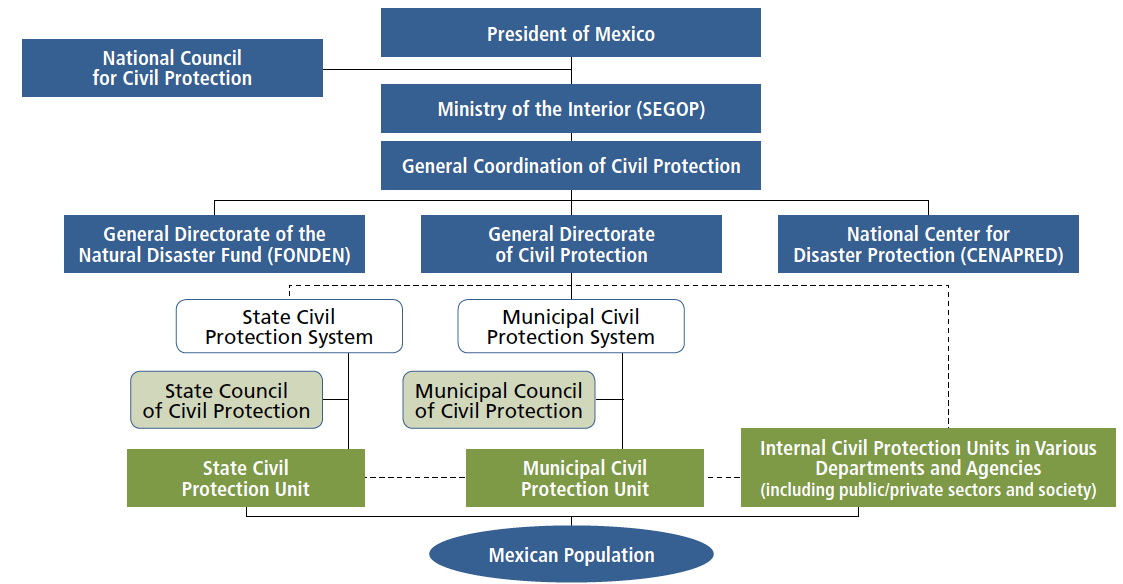
\includegraphics{img/SEGOB.png}
\caption{Flow Chart of the Civil Protection System in Mexico,
\break Source: ``FONDEN: Mexico´s Natural Disaster Fund, A Review'',
World Bank (2012)}
\end{figure}

The Mexican Civil Protection Law defines a disaster as \emph{``\ldots{}
a situation in which the population of one or more State entities
suffers several damages from the impact of a natural or man--made
disaster calamity, resulting in loss of life, infrastructure or
environment, in a way that disrupts the social structure and disturbs
the essential activities of society, affecting livelihoods.''} When a
disaster occurs, the local government (municipal and state level)
attends the disaster through the local civil protection system and a
state fund for disasters. If the disaster overwhelms local capacity, the
state government request help from SEGOB. One of the main problems is
there are no indicators nor measures for ``local capacity''.

When a disaster occurs the process of declaration is the following:
First, SEGOB must issue a declaration of a natural disaster in order for
FONDEN resources to be accessible by affected federal agencies or state
governments. Once this declaration has been made, the federal agencies
and/or state government(s) can apply for funding and the damage
assessment process. In order to ensure efficiency and accuracy of the
damage assessment process, a committee composed by CENAPRED, the
National Water Commission (CONAGUA) and the National Forestry Commission
(CONAFOR), make a report of the disaster. Based on the findings of the
damage assessment, SEGOB reviews the related funding applications,
determines the appropriate allocations, and requests the Ministry of
Finance and Public Credit (SHCP) to convene the FONDEN Technical
Committee to authorize the transfer of funds to a subaccount for the
reconstruction program in the FONDEN Trust. From this subaccount,
resources are transferred to the service providers implementing
reconstruction works. FONDEN resources finance 100 percent of the
reconstruction costs for federal assets and 50 percent of those for
local assets the first time that the assets are affected by a disaster,
afterwards the percentage of recovery declines and local government
should buy insurance for the reconstructed
assets\footnote{GFDRR (2012)}. Figure 2 explains the process to access
and execute FONDEN resources for post-disaster reconstruction.

\begin{figure}[htbp]
\centering
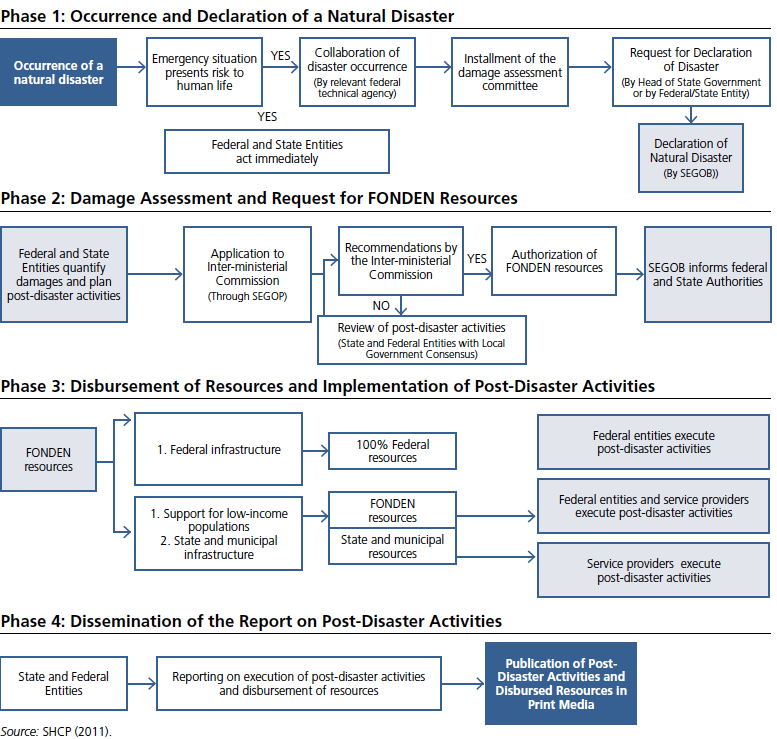
\includegraphics{img/proces.png}
\caption{Process to access and execute FONDEN resources for
post-disaster reconstruction,\break Source: ``FONDEN: Mexico´s Natural
Disaster Fund, A Review'', World Bank (2012)}
\end{figure}

\break

It is important to mention that federal disaster relief assistance is a
grant and all the system depends in the declaration made by SEGOB. If
the disaster is not declared then the state has no help from the federal
level, meaning, it only has local assistance. If the disaster is
declared, SEGOB has four types of
declaration\footnote{The type of aid depends on the type of declaration}

\begin{figure}[htbp]
\centering
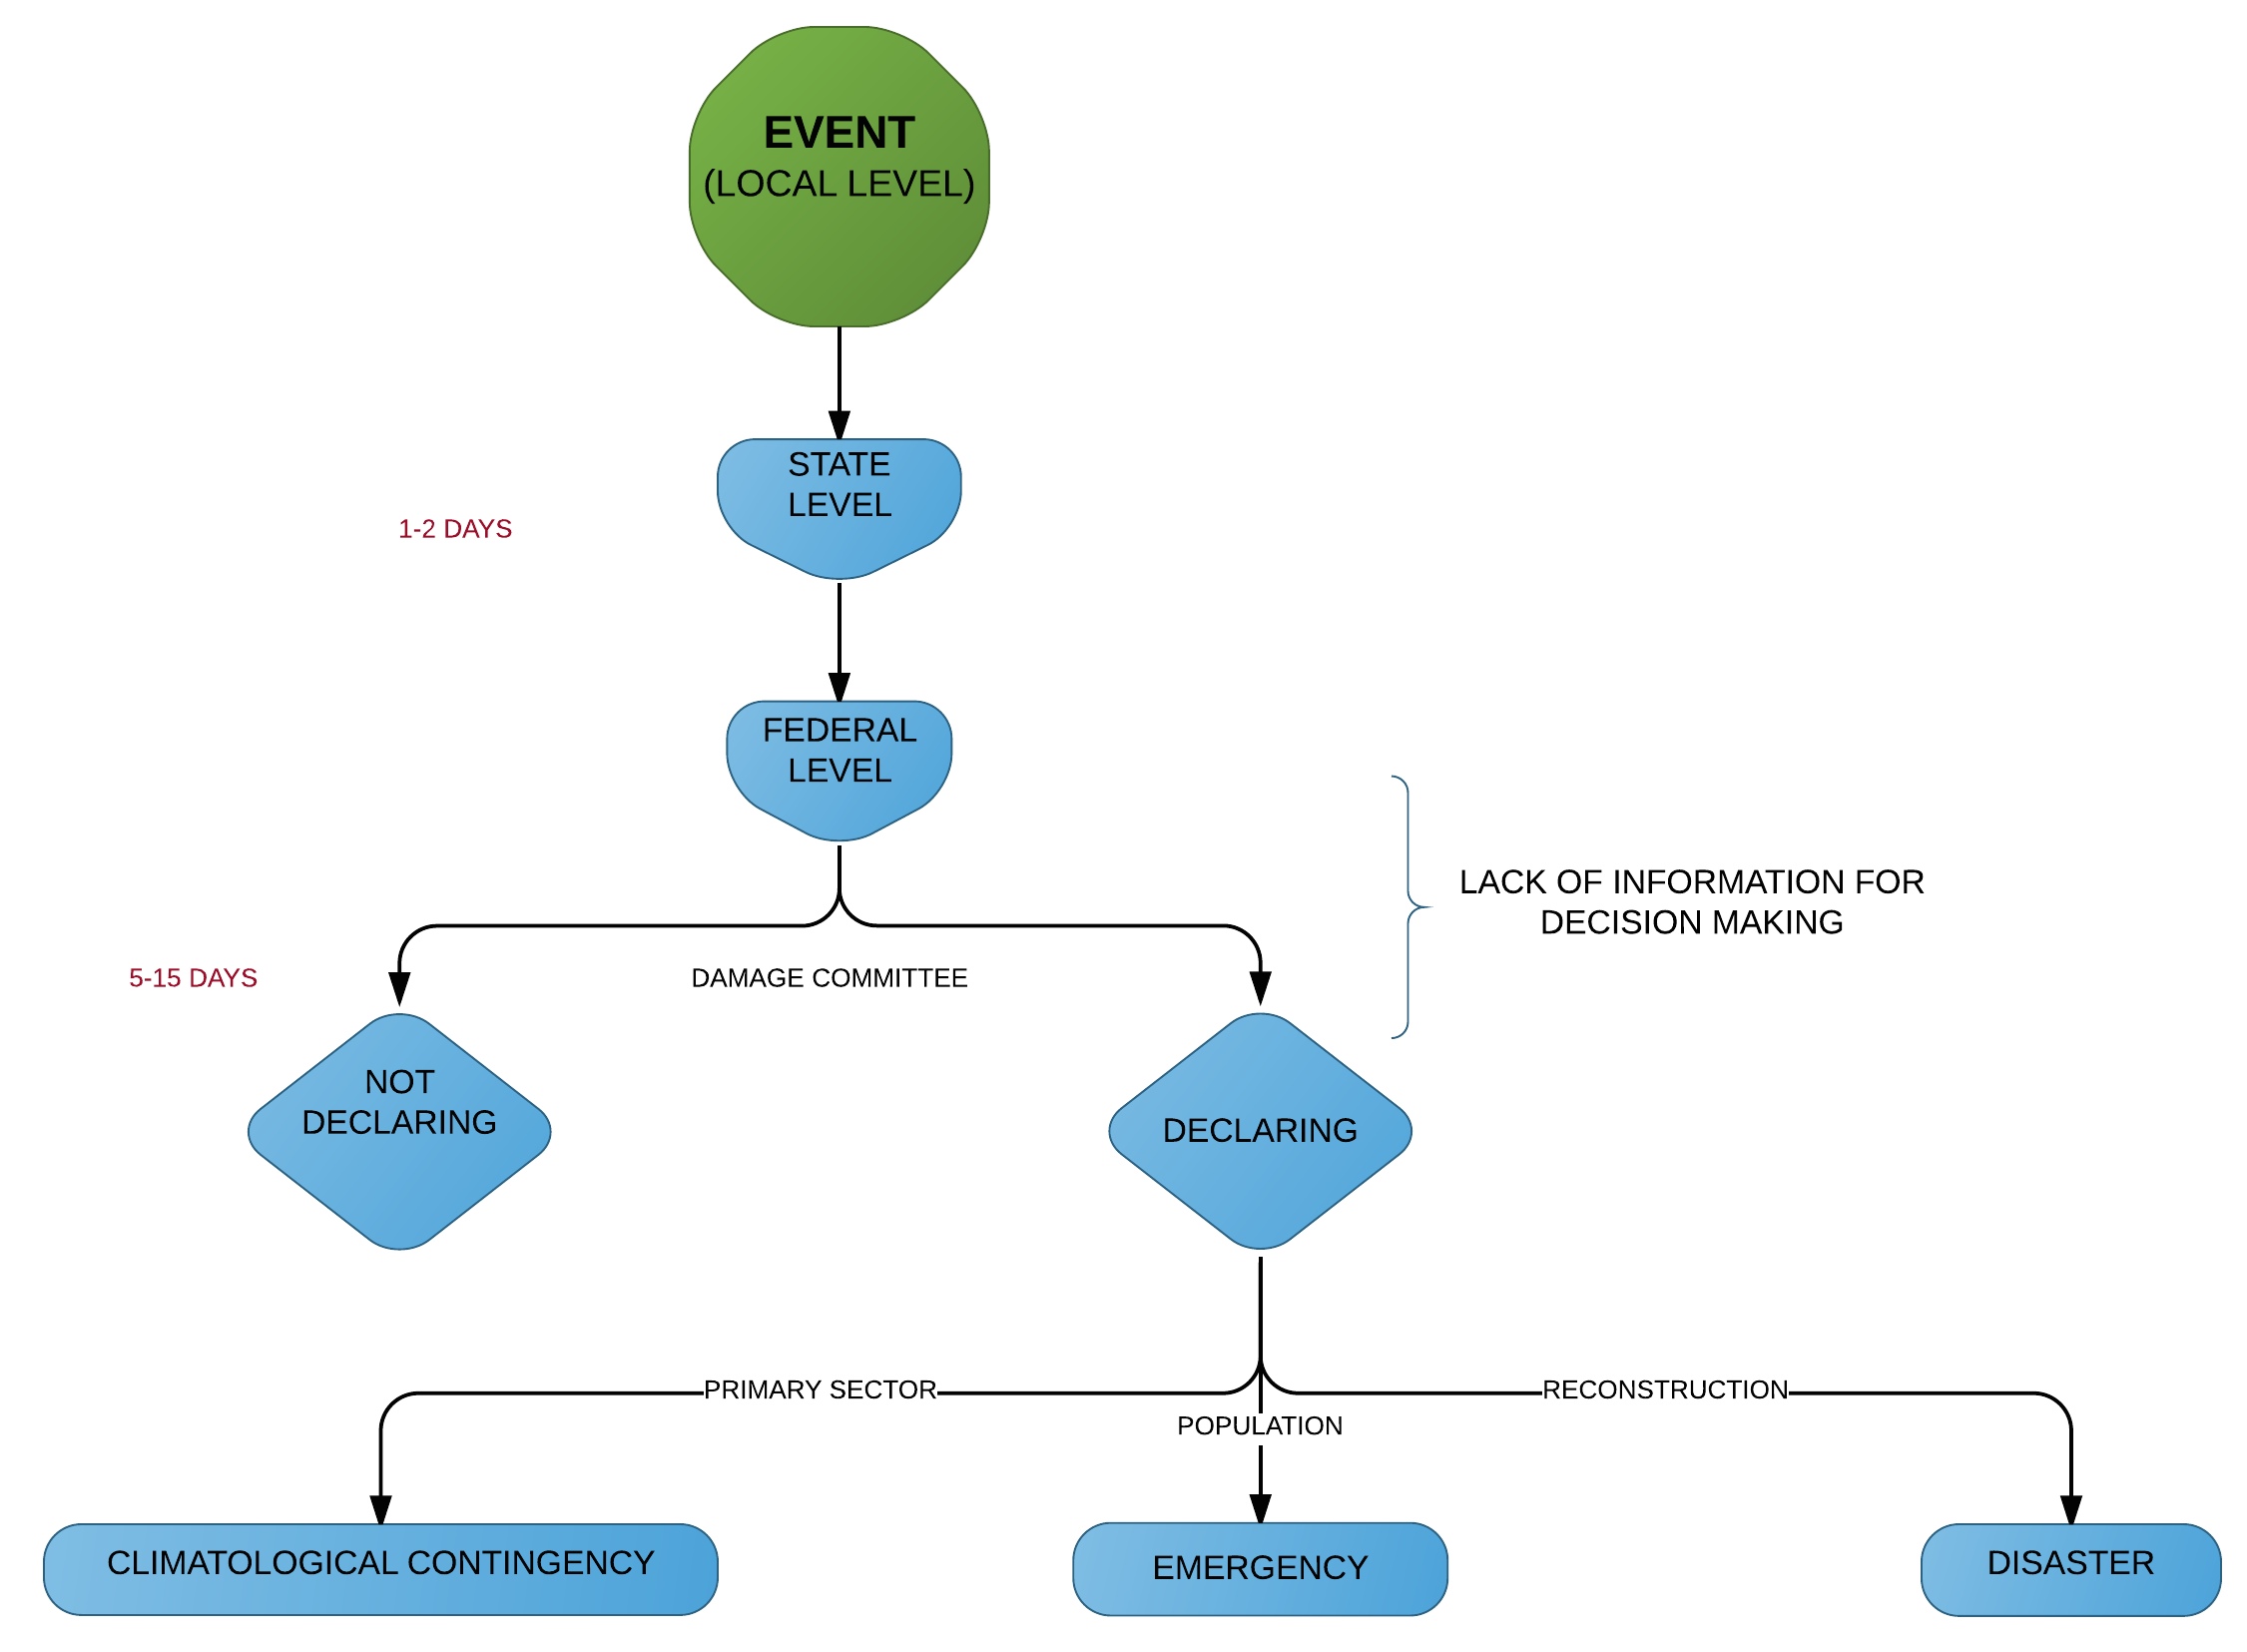
\includegraphics{img/proceso1.png}
\caption{Disaster Declaration Process}
\end{figure}

\break

\section{Research Problem}\label{research-problem}

The lack of information during and after a disaster is one of the main
problems for public policy makers for disaster mitigation and even
conflict
prevention.\footnote{Meier, Patrick. (2014). Crisis Mapping in Areas of Limited Statehood. In Information and Communication Technologies in Areas of Limited Statehood, ed. Steven Livingston and Gregor Walter-Drop. Oxford University Press}\footnote{Meier, Patrick. (2014). Human Computation for Disaster Response. In Handbook of Human Computation, ed. Pietro Michelucci et. al, Springer}
As explained above when Mexican government decide between declaring and
dot declaring a disaster they only rely on the information given by the
local governments and the meteorological data (precipitation, wind and
temperature)

\begin{figure}[htbp]
\centering
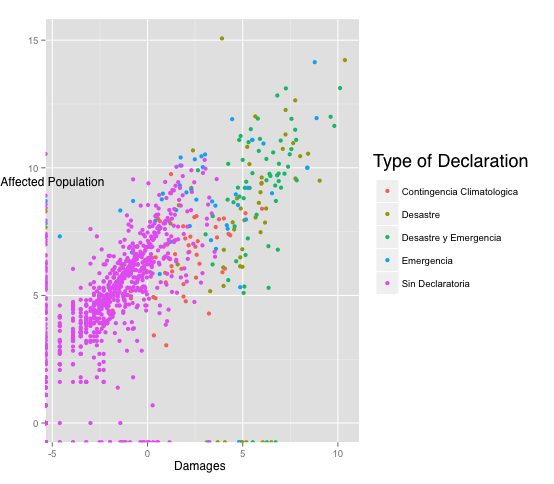
\includegraphics{img/shady.png}
\caption{Damages vs Affected Population}
\end{figure}

\section{Literature Review}\label{literature-review}

\section{Knowledge Gaps}\label{knowledge-gaps}

\section{Research Objectives}\label{research-objectives}

This project analyzes the main variables determining the Mexican process
of disaster declaration looking forward a predictor for helping Mexican
government to make a transparent process regarding disasters driven by
hydro meteorological phenomena's. The objective of this project is to
develop and apply methods to assess the suitability of using news flows
and precipitation data to characterize disaster damages in Mexico
looking forward to resource allocation improvement.

The extension of the project depends of the data needed and gathered. As
mentioned above we will work towards an open, real time visualization
platform for coordinated disaster mitigation for decision-making.

\break 

\section{Data}\label{data}

The period of study is 2002-2013. The following section describes the
data groups needed for this project:

\begin{figure}[htbp]
\centering
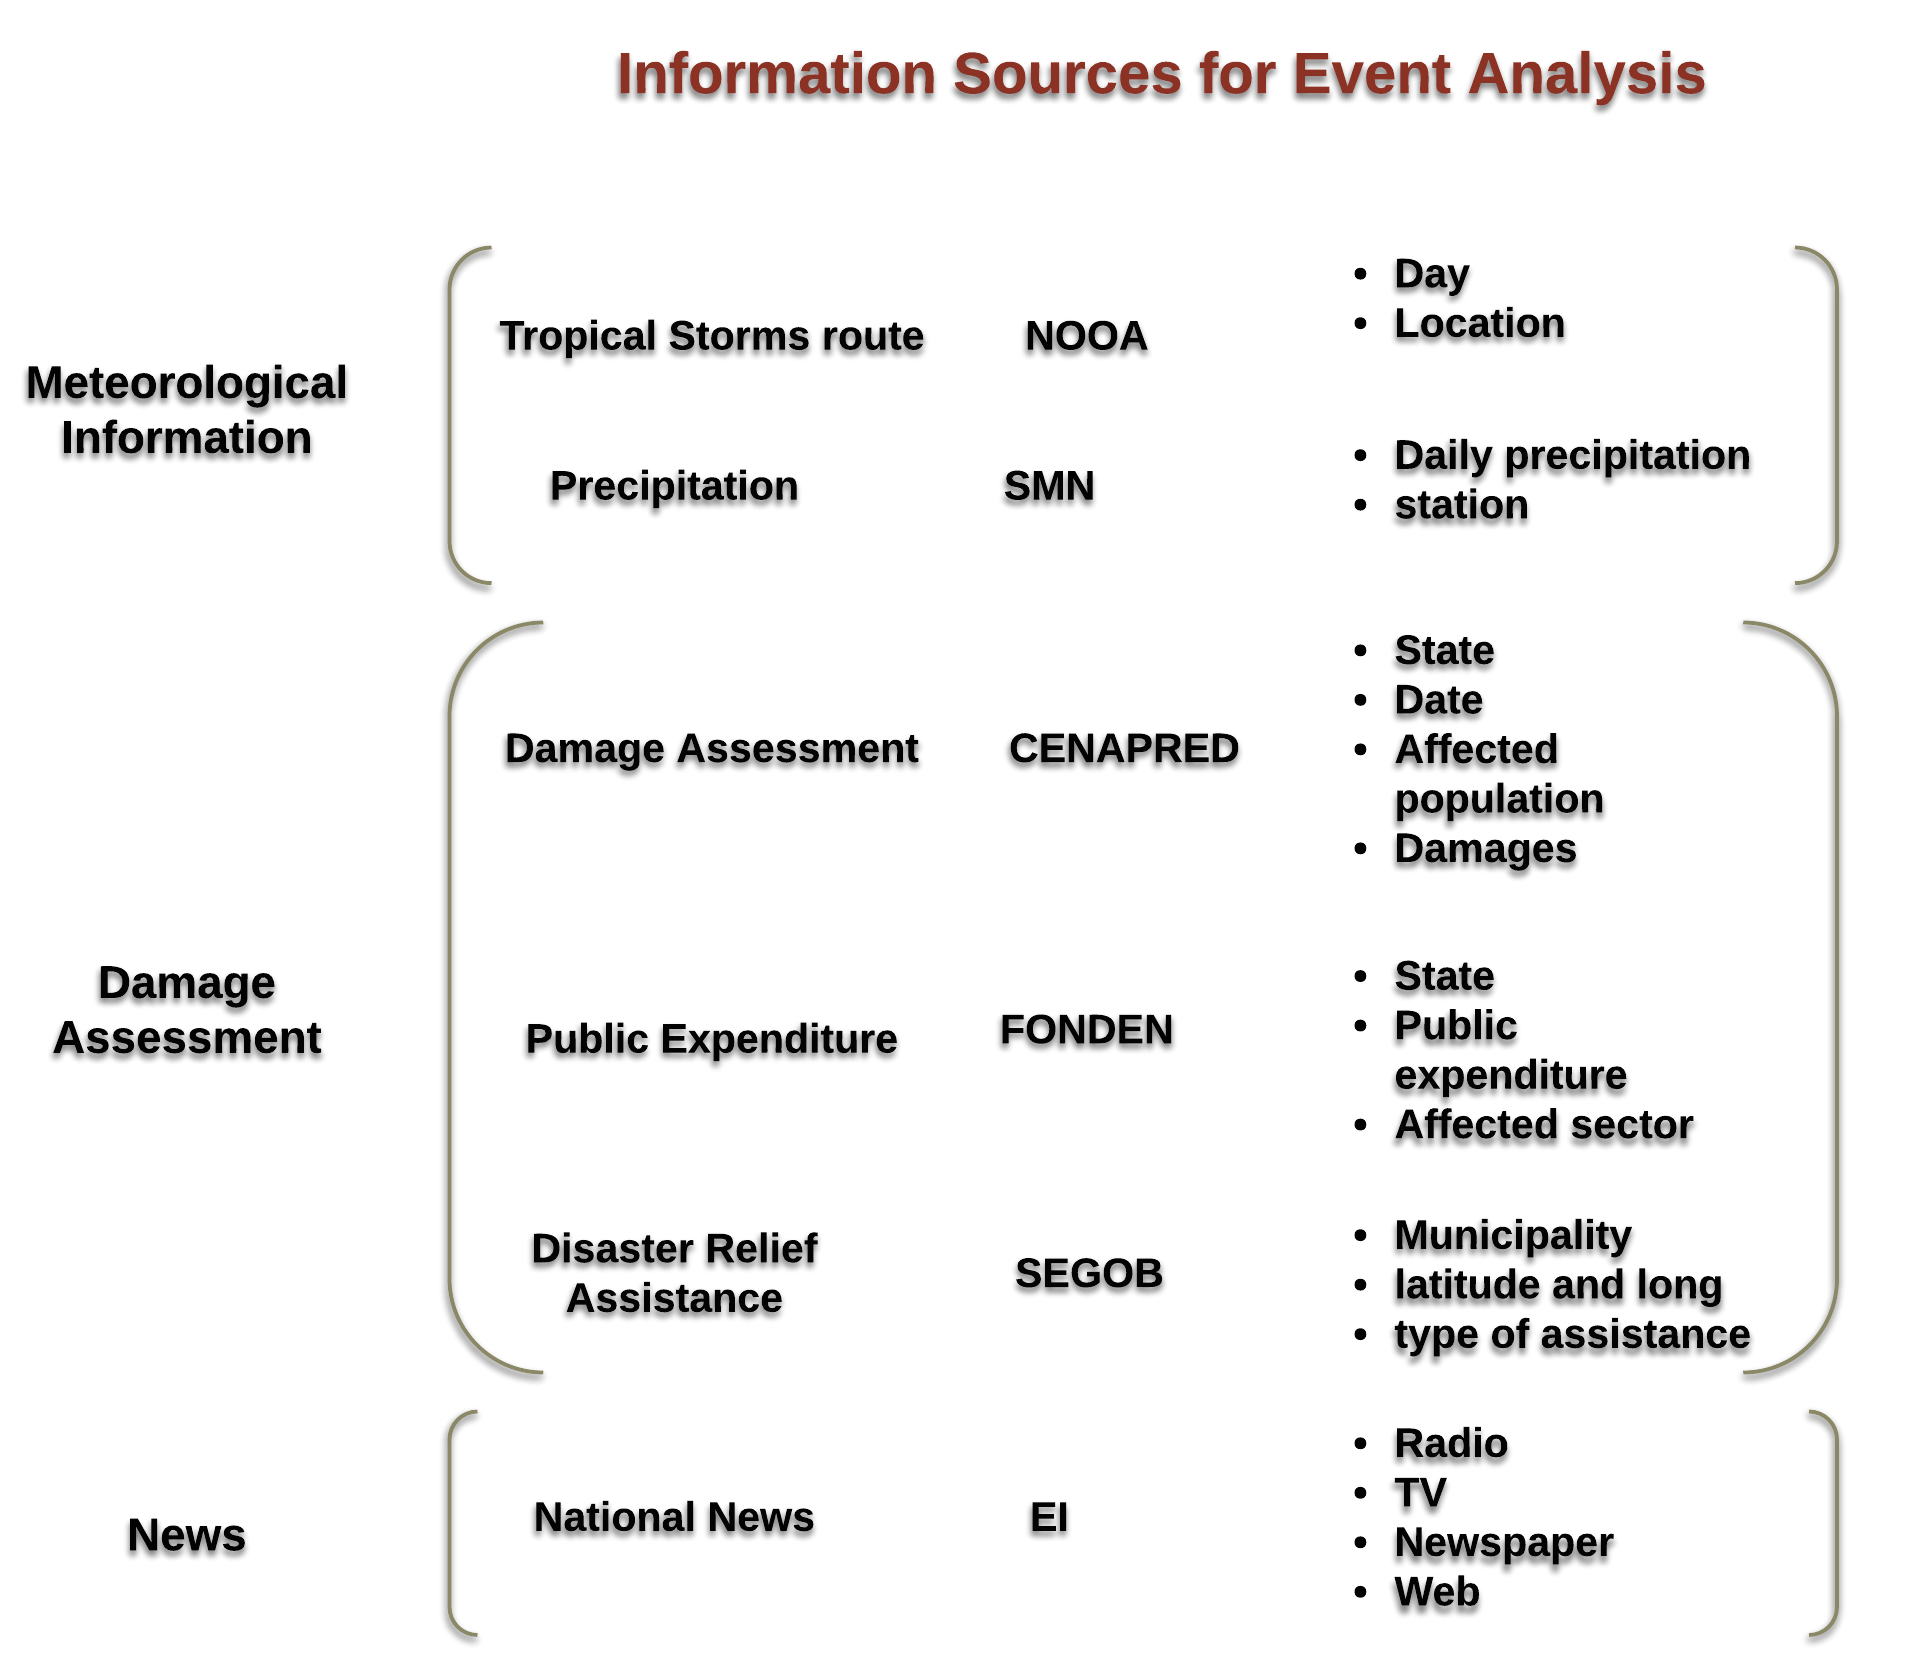
\includegraphics{img/sources.png}
\caption{Sources}
\end{figure}

\break

\begin{itemize}
\itemsep1pt\parskip0pt\parsep0pt
\item
  \textbf{News data}: The Company ``Eficiencia Informativa''
  \href{http://data4.efinf.com/reader/web/}{EI} gathers information from
  electronic, newspaper, radio and TV news. The idea is to scrap all the
  news related to climatic events during the period of study. The
  company gave an acces for using their information till the endo of the
  year.
\end{itemize}

\begin{figure}[htbp]
\centering
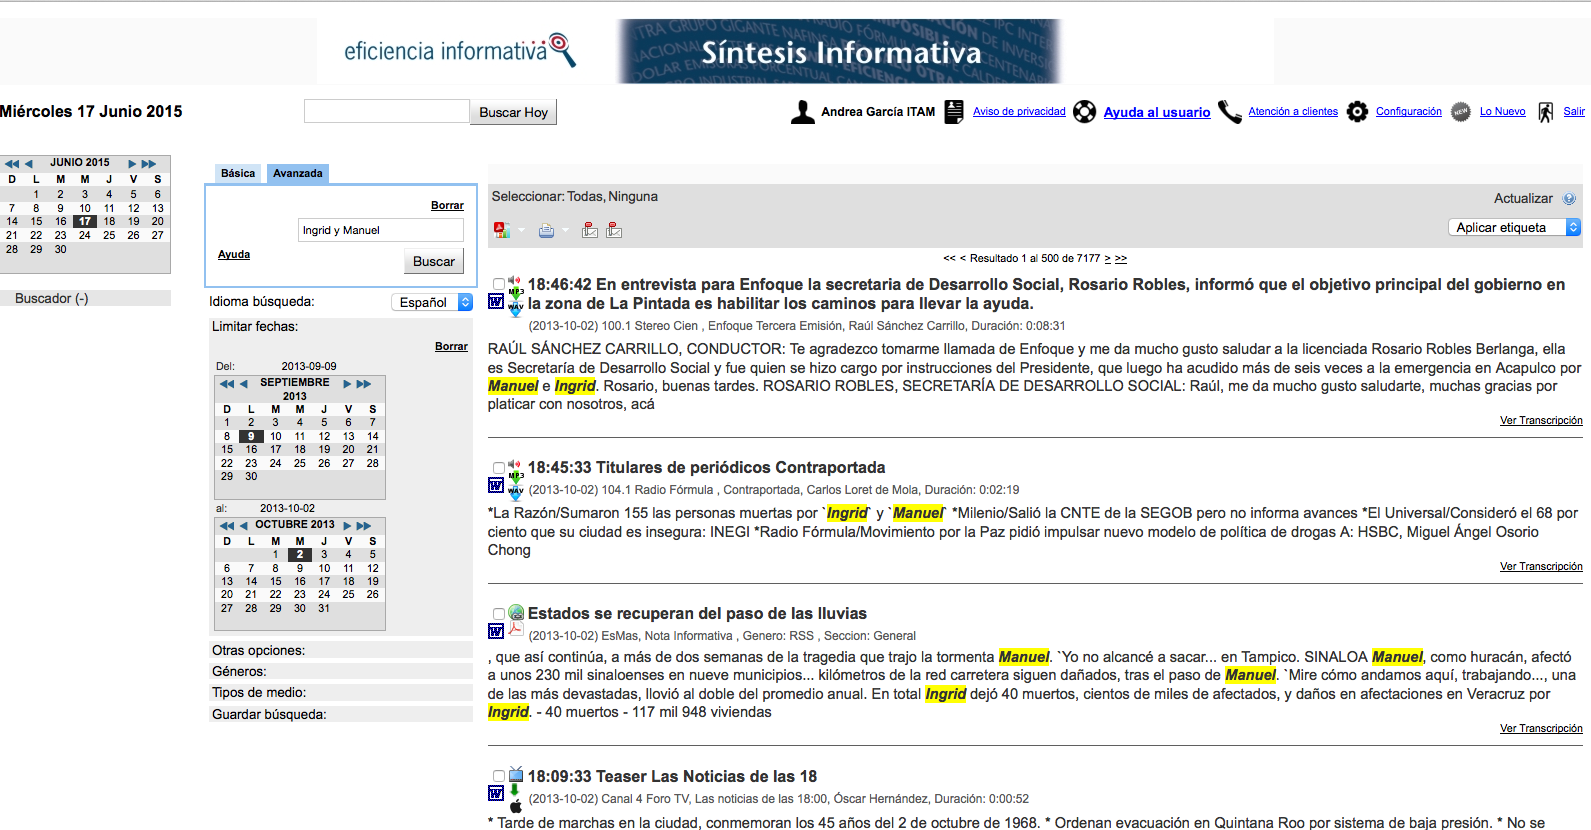
\includegraphics{img/EI.png}
\caption{Eficiencia Informativa System}
\end{figure}

They have different formats for downloading the information. The best is
CSV

\begin{figure}[htbp]
\centering
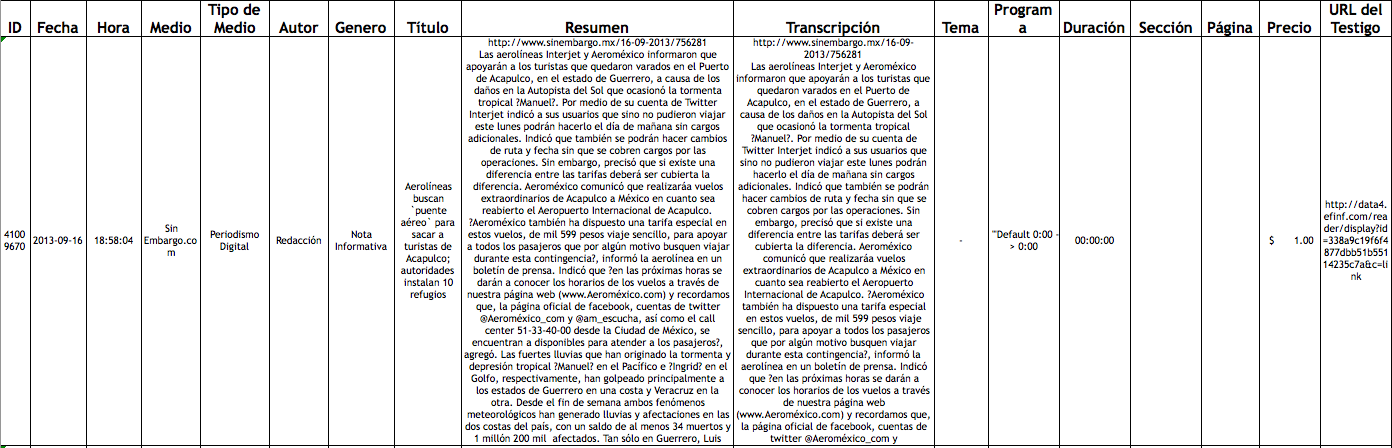
\includegraphics{img/EI_prueba.png}
\caption{Example of the DB}
\end{figure}

\begin{itemize}
\itemsep1pt\parskip0pt\parsep0pt
\item
  \textbf{Disaster Database}:

  \begin{itemize}
  \item
    \emph{Disaster Evaluation}: The National Center for Natural Disaster
    Prevention (CENAPRED) is in charge of the disaster damage and loss
    evaluation for the affected states. They gave us an access to the
    National Risk Atlas
    \href{http://atlasnacionalderiesgos.gob.mx/}{ANR} and the evaluation
    dataset. Since Ingrid and Manuel Storms affected 19 of the 31
    mexican states the government could not make a comprehensive damage
    evaluation. They were only able to do 5 damage evaluations (Durango,
    Guerrero, Nuevo Leon, Sianloa and Veracruz ). The access to the ANR
    is not working so good since an older versión of explorer is needed.
    We are trying to access the platform in other system.
    \footnote{if the acces is not working next week we will procede to ask for each data base}
  \item
    \emph{Public Spending}: The Ministry of Interior(SEGOB) manages the
    Disaster Relief Fond (FONDEN) through the National Civil Protection
    Service
    (SINAPROC)\footnote{For more information about FONDEN system see Garcia, A. (2014) "Desastres Naturales: Destrucción Creativa?",Chapter2, BA thesis ITAM}.
    The public spending records are available online
    \href{http://www.proteccioncivil.gob.mx/es/ProteccionCivil/Recursos_Autorizados_por_Declaratoria_de_Desastre}{Recursos
    Autorizados}. Ingrid y Manuel disasters have a lag of 3 years of
    public spending. Each year has diferent format and information. We
    are working on the data cleaning. For following up the disasters,
    SEGOB opend a platform to inform the reconstruction actions and the
    money expeded
    \href{http://www.presidencia.gob.mx/fonden/}{Presidencia}. The data
    in this platform does not match with the data obtained in FONDEN web
    site in spite of being the same govenrment entity. We already send a
    mail asking for this inconsistencies.
  \end{itemize}
\end{itemize}

\begin{figure}[htbp]
\centering
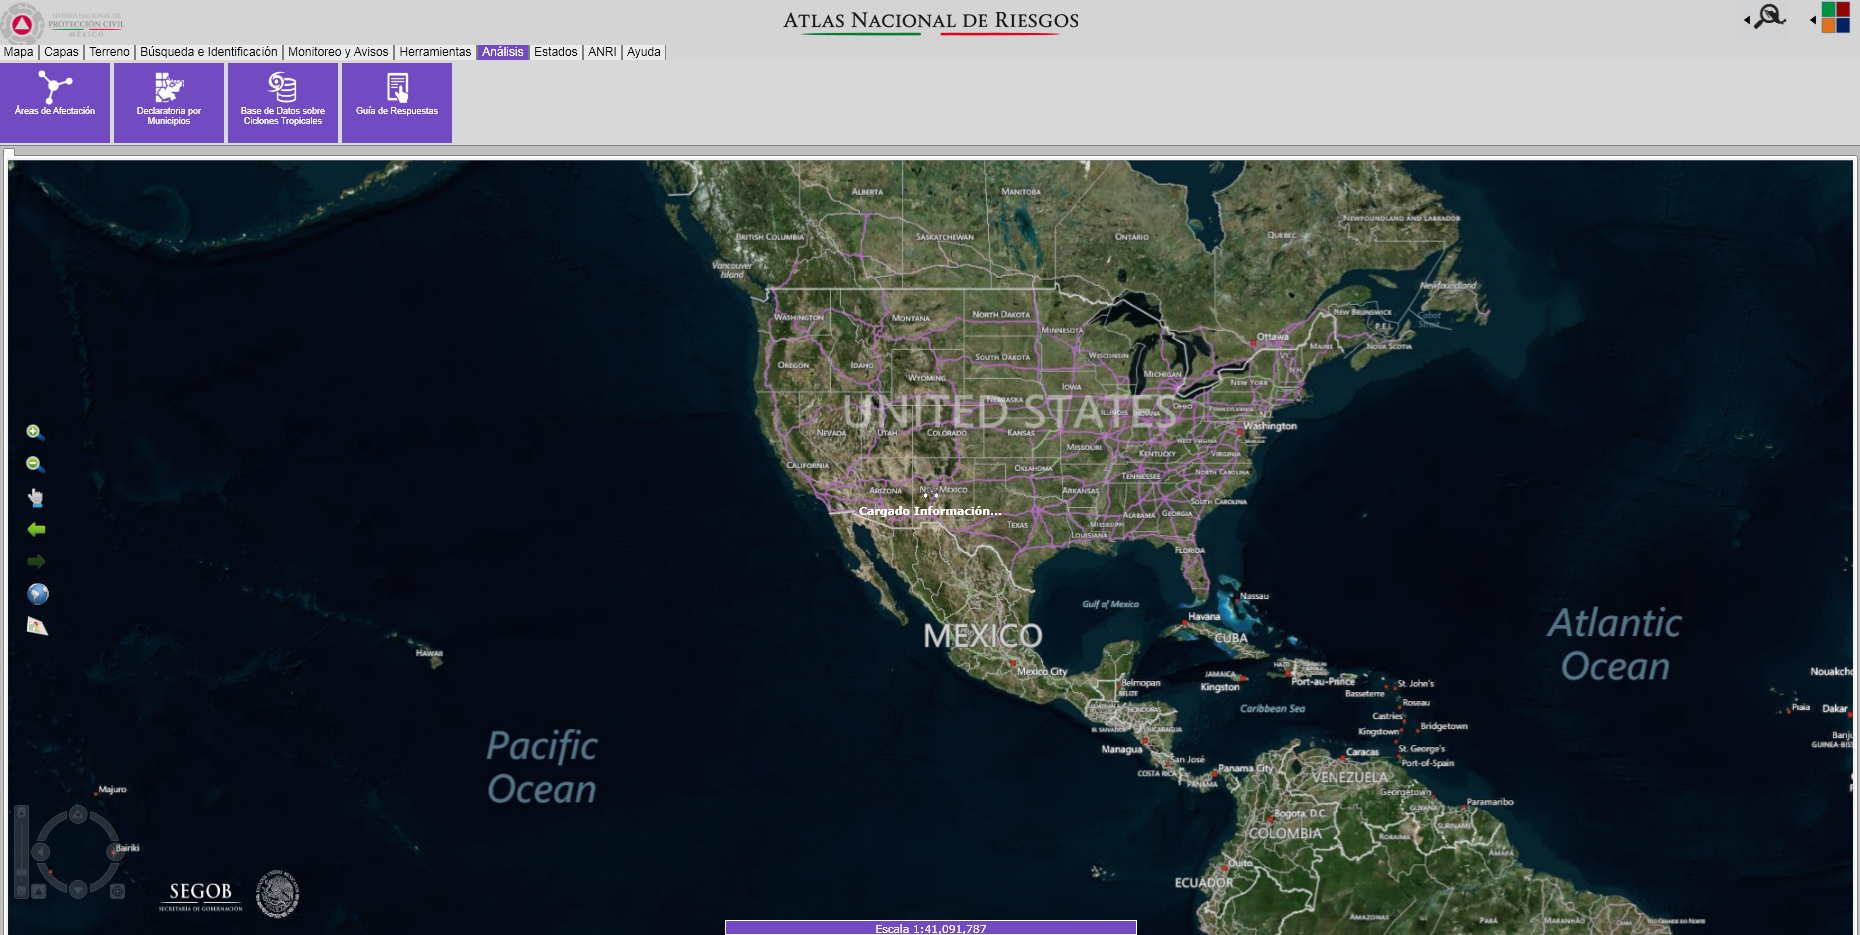
\includegraphics{img/anr.png}
\caption{National Risk Atlas}
\end{figure}

\begin{itemize}
\itemsep1pt\parskip0pt\parsep0pt
\item
  \textbf{Meteorological Information}: The precipitation data could help
  us as a proxy for damage metrics. The data could be obtained by NASA
  precipitation grid or by the National Meteorological System.
\end{itemize}

\section{Methodology}\label{methodology}

++Intro clasificadores++

To clasify the types of delcarations a Support Vector Machine and a
Random Forest will be used\ldots{}

\subsection{News mining}\label{news-mining}

In the news dataset we have the transcripts of the news on TV, radio and
newspapers. Radio transcripts are smaller than the TV or newspaper
transcripts so for the text mining processing we need a methodology that
allow us to search for the relevant (more frequent words) weighting the
extension of the transcript and using stop words.

The idea is to do text mining for processing this database and follow
the coverage of the disasters in the news.

\begin{figure}[htbp]
\centering
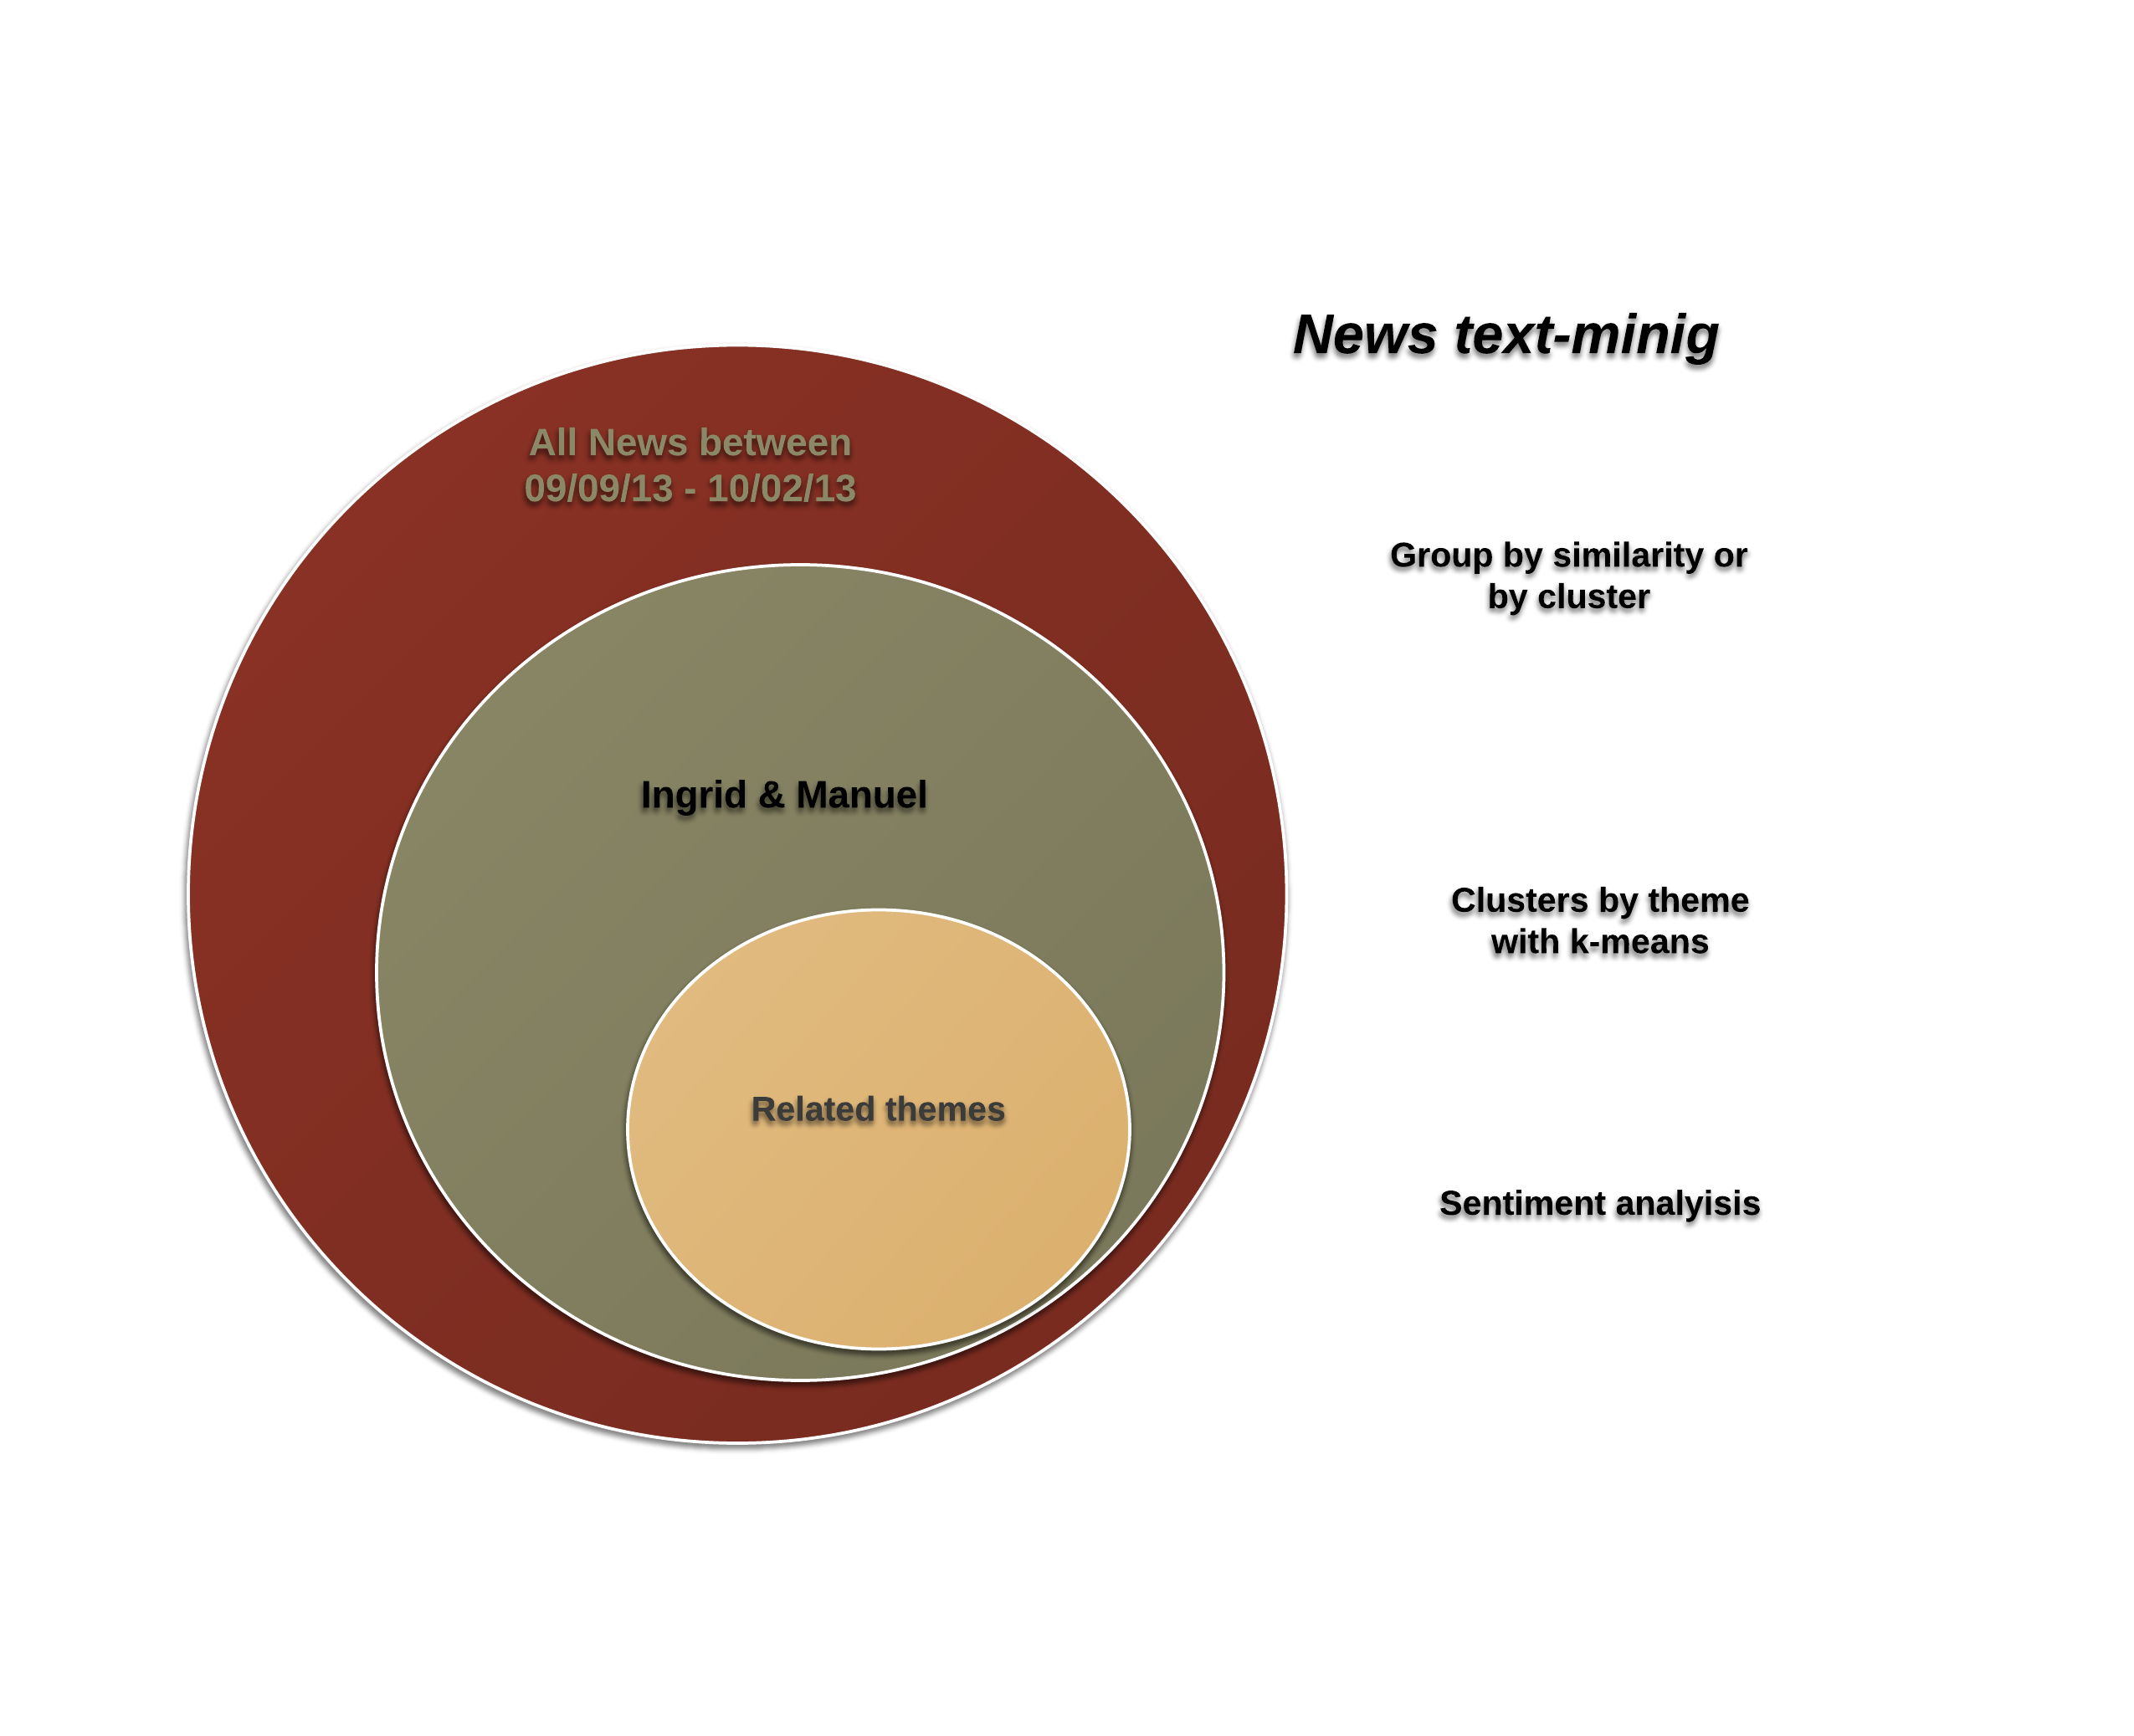
\includegraphics{img/news.png}
\caption{Example news procesing}
\end{figure}

+++++++++++++++++++++++++++++++++++++++++++ Como se mencionó
anteriormente , no basta con filtrar las noticias según la aparición de
las palabras clave, ni tampoco un conteo simple. se podría tomar en
cuenta los conteos, pero usando técnicas para disminuir la importancia
de la longitud de los documentos y de la frecuencia de aparición de las
palabras comunes.

Denotamos la frecuencia del término $w$ (puede ser una palabra o la raíz
de una palabra obtenida con \emph{stemming}) en el documento $d$ como
$tf_{w,d}$. De manera natural, denotamos por $tf_d$ al vector de todas
las frecuencias de los términos conocidos del documento $d$. Supongamos
que queremos comparar los documentos $q$ y $d$. Un primer enfoque que
podríamos utilizar sería usar la distancia coseno, que toma en cuenta
únicamente la frecuencia relativa de las palabras dentro de los
documentos:

\[
d_{coseno}(q,d) = \frac{tf_q \cdot tf_d}{\|tf_q\| \|tf_d\|}
\]

El problema con lo anterior es que las palabras comunes podrían tomar un
papel protagónico y en nuestro caso compartir por ejemplo artículos o
preposiciones no es muy interesante. Para mitigar esto utilizaremos la
frecuencia inversa en documentos $idf_w$, definida para una palabra $w$.
Si $N$ es el número total de documentos en la colección y $df_w$ es el
número de documentos de la colección que contienen a $w$, entonces
definimos la frecuencia inversa de documentos como sigue:

\[
idf_w = log(\frac{N}{df_w}) 
\]

Y entonces, en lugar de describir a $d$ por medio de $tf_d$, lo
describimos por medio de $c_d$, donde

\[
c_{d,w} = idf_w \times tf_{d,w}
\]

Y así, calculamos la distancia entre dos documentos como la distancia
coseno entre sus vectores característicos:

\[
d(q,d) = \frac{c_q \cdot c_d}{\|c_q\| \|c_d\|}
\]

La $idf_w$ es el logaritmo del inverso de la probabilidad de que el
término $w$ aparezca en un documento elegido al azar. El efecto que esto
tiene es que las palabras comunes casi no tendrán ningún efecto en la
distancia, puesto que su probabilidad es cercana a 1 y por lo tanto su
$idf$ es cercana a cero. Por el contrario, las palabras raras tendrán
una probabilidad cercana a 0, por lo que su $idf$ será grande y
contribuirán mucho. La razón detrás de hacer esto es que queremos que
discriminen las palabras especiales o específicas a un contexto y no las
genéricas. El esquema expuesto está escrito con mayor detalle en el
libro \href{http://www.mmds.org}{Mining of Massive Datasets}, con la
pequeña diferencia de que ahí además normalizan $tf_w$ por la máxima
frecuencia obtenida por el término en la colección de documentos.

\emph{Indicador de Noticias}

Plan A

Procesar todas las noticias en el periodo de estudio y sacar los temas
relevantes en las fechas de desastres y ver si tuvo impacto en las
noticias

Plan B Porcesar solo las noticias relacionadas a palabras clave
relacionadas a eventos climáticos

++Pedir asesoría al profesor Luis Felipe Gonzalez+++

++++++++++++++++++++++++++++++++++++++++++

\section{Results}\label{results}

\section{Conclusion}\label{conclusion}

\section{Further Investigation}\label{further-investigation}

\section{Bibliography}\label{bibliography}

\begin{enumerate}
\def\labelenumi{\arabic{enumi}.}
\itemsep1pt\parskip0pt\parsep0pt
\item
  Caragea et al, (2011). Classifying text messages for the Haiti
  earthquake. Proceedings of the 8th International Conference on
  Information Systems for Crisis Response and Management (ISCRAM2011).
\item
  CENAPRED (2010) Serie de Impacto Socioeconomico
  www.atlasnacionalderiesgo.gob.mx
\item
  Chew C \& Eysenbach G (2010) Pandemics in the Age of Twitter: Content
  Analysis of Tweets during the 2009 H1N1 Outbreak. PLoS ONE
  5(11):e14118.
\item
  Christakis, Nicholas A. Y James H. Fowler (2010). ``Social Network
  Sensors for Early Detection of Contagious Outbreaks'',
  \url{http://www.plosone.org/article/info\%3Adoi\%2F10.1371\%2Fjournal.pone.0012948}
\item
  Chunara R, Andrews JR, \& Brownstein JS (2012) Social and News Media
  Enable Estimation of Epidemiological Patterns Early in the 2010
  Haitian Cholera Outbreak. The American Journal of Tropical Medicine
  and Hygiene 86(1):39-45.
\item
  CONAGUA(2014), ``Reporte del Clima en México 2013'', Coordinación
  General del Servicio Meteorológico Nacional. 06/11/15,
  \url{http://www.conagua.gob.mx}
\item
  Earle PS, Bowden DC, \& Guy M (2012) Twitter earthquake detection:
  earthquake monitoring in a social world. Annals of Geophysics
  54(6):708-715.
\item
  FONDEN, Recursos Autorizados por Declaratoria de Desastre. 06/12/15,
  \url{http://www.proteccioncivil.gob.mx/es/ProteccionCivil/Recursos_Autorizados_por_Declaratoria_de_Desastre}
\item
  Freeman M (2011) Fire, wind and water: Social networks in natural
  disasters. Journal of Cases on Information Technology (JCIT) 13(2):
  69-79.
\item
  Gao, H, Barbier, G. and Goolsby R. Harnessing the crowdsourcing power
  of social media for disaster relief (2011). DTIC Document.
\item
  Garcia A (2014) ¿Desastres naturales: destrucción creativa? Bachelor
  Thesis ITAM
\item
  Garcia A, Muñoz C (2014) The Effect of Natural Disasters on Mexico's
  Regional Economic Growth: Growing Disparity or Creative Destruction?
  Working Paper Series, WP68 Latin American and Caribbean Environmental
  Economics Program (LACEEP), available at :
  \url{http://www.laceep.org/index.php?option=com_k2\&view=item\&id=226:the-effect-of-natural-disasters-on-mexico\%E2\%80\%99s-regional-economic-growth-growing-disparity-or-creative-destruction}?-andrea-garc\&Itemid=87
\item
  Guan X \& Chen C (2014) Using social media data to understand and
  assess disasters. Natural Hazards:1-14.
\item
  Guy M, Earle P, Ostrum C, Gruchalla K, \& Horvath S (2010) Integration
  and dissemination of citizen reported and seismically derived
  earthquake information via social network technologies. Advances in
  intelligent data analysis IX, (Springer), pp 42-53.
\item
  Henry D, Ramirez-Marquez JR. (2012) Generic metrics and quantitative
  approaches for system resilience as a function of time. Reliability
  Engineering and System Safety; 99(1):114--122.
\item
  Herfort B, de Albuquerque JP, Schelhorn S-J, \& Zipf A (2013) Does the
  spatiotemporal distribution of tweets match the spatiotemporal
  distribution of flood phenomena? A study about the River Elbe Flood in
  June 2013.
\item
  Hughes AL \& Palen L (2009) Twitter adoption and use in mass
  convergence and emergency events. International Journal of Emergency
  Management 6(3):248 260.
\item
  Imran M, Elbassuoni SM, Castillo C, Diaz F, \& Meier P (2013)
  Extracting information nuggets from disaster-related messages in
  social media. Proc. Of ISCRAM, Baden-Baden, Germany.
\item
  Kryvasheyeu Y, Chen H, Moro E, Van Hentenryck P, \& Cebrian M (2015)
  Performance of Social Network Sensors during Hurricane Sandy. PLoS ONE
  10(2):e0117288.
\item
  Kumar S, Hu X, \& Liu H (2014) A behavior analytics approach to
  identifying tweets from crisis regions. Proceedings of the 25th ACM
  conference on Hypertext and social media, (ACM), pp 255-260.
\item
  Li J \& Rao H (2010) Twitter as a rapid response news service: An
  exploration in the context of the 2008 China Earthquake. The
  Electronic Journal of Information Systems in Developing Countries
  42(4):1-22.
\item
  Meier, P. (2014) Crisis Mapping in Areas of Limited Statehood. In
  Information and Communication Technologies in Areas of Limited
  Statehood, ed. Steven Livingston and Gregor Walter-Drop. Oxford
  University Press
\item
  Meier, P. (2014) Human Computation for Disaster Response. In Handbook
  of Human Computation, ed. Pietro Michelucci et. al, Springer.
\item
  Meier, P. (2014) Using Advanced Computing to Verify User-Generated
  Content on Social Media, in The Verification Handbook, eds. Craig
  Silverman and Rina Tsubaki.
\item
  Myers SA, Sharma A, Gupta P, \& Lin J (2014) Information network or
  social network?: the structure of the twitter follow graph.
  Proceedings of the companion publication of the 23rd international
  conference on World wide web companion, (International World Wide Web
  Conferences Steering Committee), pp 493-498.
\item
  National Hurricane Center, NOAA. 06/11/15,
  \url{http://www.nhc.noaa.gov/aboutsshws.php}
\item
  Power R, Robinson B, Colton J, \& Cameron M (2014) Emergency Situation
  Awareness: Twitter Case Studies. Information Systems for Crisis
  Response and Management in Mediterranean Countries, Lecture Notes in
  Business Information Processing, eds Hanachi C, Bénaben F, \& Charoy F
  (Springer International Publishing), Vol 196, pp 218-231.
\item
  Preis T, Moat HS, Bishop SR, Treleaven P, \& Stanley HE (2013)
  Quantifying the Digital Traces of Hurricane Sandy on Flickr. Sci.
  Rep.~3:3141.
\item
  Protección Civil. 06/15/15,
  \url{http://www.proteccioncivil.gob.mx/es/ProteccionCivil/Apoyos_otorgados_2013}
\item
  Ramirez-Marquez JE, Rocco CM. (2009) Stochastic network interdiction
  optimization via capacitated network reliability modeling and
  probabilistic solution discovery. Reliability Engineering and System
  Safety; 94(5):913--921.
\item
  Sakaki T, Okazaki M, \& Matsuo Y (2010) Earthquake shakes Twitter
  users: real-time event detection by social sensors. Proceedings of the
  19th international conference on World wide web: 851-860.
\item
  Servicio Meteorológico Nacional (SMN). 06/10/15,
  \url{http://smn.cna.gob.mx/index.php?option=com_content\&view=article\&layout=edit\&id=268}
\item
  Skinner J (2013) Natural disasters and Twitter: Thinking from both
  sides of the tweet. First Monday; Volume 18, Number 9 - 2 September
  2013.
\item
  Takahashi, Tetsuro, Shuya Abe y Nobuyuki Igata (2011). ``Can Twitter
  Be an Alternative of Real-World Sensors?'' Human-Computer Interaction.
  Towards Mobile and Intelligent
\item
  Topsy Labs (2012), Topsy website. Available:
  \url{http://www.topsylabs.com}, Accessed 2012 November 20
\item
  Tropical Cyclone Report. Hurricane Sandy (AL182012) 22 -- 29 October
  2012 (2013). National Hurricane Center.
\item
  Van Hentenryck P (2013) Computational disaster management. Proceedings
  of the Twenty- Third international joint conference on Artificial
  Intelligence, (AAAI Press), pp 12-18.
\item
  Vieweg S, Hughes AL, Starbird K, \& Palen L (2010) Microblogging
  during two natural hazards events: what twitter may contribute to
  situational awareness. Proceedings of the SIGCHI Conference on Human
  Factors in Computing Systems, (ACM), pp 1079-1088.
\item
  Wang D, Lin Y-R, \& Bagrow JP (2012) Social Networks in Emergency
  Response. Encyclopedia of Social Network Analysis and Mining).
\item
  Wang Q \& Taylor JE (2014) Quantifying Human Mobility Perturbation and
  Resilience in Hurricane Sandy. PLOS ONE 9(11):e112608.
\item
  Watts D, Cebrian M, \& Elliot M (2013) Dynamics of Social Media.
  Public Response to Alerts and Warnings Using Social Media: Report of a
  Workshop on Current Knowledge and Research Gaps, (The National
  Academies Press), pp 22-33.
\item
  World Bank (2012) FONDEN: Mexico's Natural Disaster Fund -- A Review.
\item
  World Bank (2013) World Development Report 2014: Risk and
  Opportunity---Managing Risk for Development. Washington, DC: World
  Bank
\end{enumerate}

\end{document}
